\documentclass{article}
\usepackage[utf8]{inputenc}
\usepackage[spanish]{babel}
\usepackage{listings}
\usepackage{graphicx}
\graphicspath{ {images/} }
\usepackage{cite}

\begin{document}

\begin{titlepage}
    \begin{center}
        \vspace*{1cm}
            
        \Huge
        \textbf{Proyecto Final}
            
        \vspace{0.5cm}
        \LARGE
        Juego Némesis
            
        \vspace{1.5cm}
            
        \textbf{Carolina Jimenez Restrepo}\\
        \textbf   { c.c 1020470694}
          \\  Grupo 3
            
            \vspace{2.9cm}
         
                   profesor: Augusto Enrique Salazar Jimenez
                   Curso: Informática II
        \vfill
            
        \vspace{0.8cm}
            
        \Large
        Despartamento de Ingeniería Electrónica y Telecomunicaciones\\
        Universidad de Antioquia\\
        Medellín\\
        Marzo de 2021
            
    \end{center}
\end{titlepage}

\tableofcontents
\newpage
\section{Sección introductoria}\label{intro}
Inspirado en el juego de mesa batalla naval, este juego se desarrolla en tierra.\\
Hace muchos años debido a las malas costumbres de los humanos, se fueron extinguiendo los recursos, los gobiernos cayeron y una crisis mundial azotó a la tierra que ahora no es habitable.
Luego de muchísima muerte y destrucción, se acabó el agua y la comida.  Los pocos humanos sobrevivientes presenciaron una terrible explosión que destruyó lo que quedaba de nuestro planeta y se vieron obligados a habitar el planeta Marte el cual no posee gravedad adaptándose a los pocos recursos que habían allí.\\
En este planeta todos luchan por sobrevivir, debido esto, se da una guerra de naves espaciales, cada uno luchando por el territorio para poder habitarlo completamente.
Todo esto siendo consecuencia del egoísmo humano que, durante muchos años y poco a poco destruyo nuestra casa.\\
"vivimos en carne propia la némesis que los dioses infligían a los mortales dominados por la soberbia"


\section{Ideas de realizacion}
\label{contenido}
\subsection{Idea principal}

El juego se llama Némesis, el objetivo es crear una estrategia que permita ubicar las naves propias en posiciones que permitan disparar al mayor numero de naves enemigas y con esa misma ubicacion cuidarse de ser atacado.

\subsection{Dideño del juego}
El desarrollo del juego es dos equipos o bandos se enfrentan con sus naves, cada equipo tiene una cantidad de naves y de disparos, la pantalla del juego se divide en dos para así tener los dos equipos y la o las personas que están jugando puedan interactuar escogiendo las posiciones de sus naves, puede ser jugado por una sola persona que controle los dos equipos o por dos personas en un equipo cada una.\\
Las naves tienen unos puntajes definidos que se van acumulando cada que reciba un disparo del enemigo, el jugador deberá usar su estrategia para ubicar las naves y así poder defenderse y atacar mejor al enemigo, cada nave tiene un nombre y podrá ser ubicada donde el jugador lo prefiera dentro del espacio de juego, se tendrá un botón para disparar, se debe escoger el ángulo con que se quiere lanzar el disparo y el movimiento que tendrá el recorrido del disparo. Cada que se agotan las balas de los dos equipos se pasa de nivel y se van desapareciendo las naves hasta que uno de los dos equipos aniquile todas las naves enemigas.\\
Los puntajes dependen del tamaño y modelo de las naves, un posible pontaje seria:\\
Nave mas grande 35 puntos\\
Nave mediana 25 puntos\\
Nave normal 40 puntos\\
Nave pequeña 50 puntos\\
El juego se desarrolla en el entorno Qt y su realizacion contara con varias clases que permitan crear cada una de las acciones necesarias para el correcto funcionamiento.\\
esquema del juego: 


\begin{figure}[h]
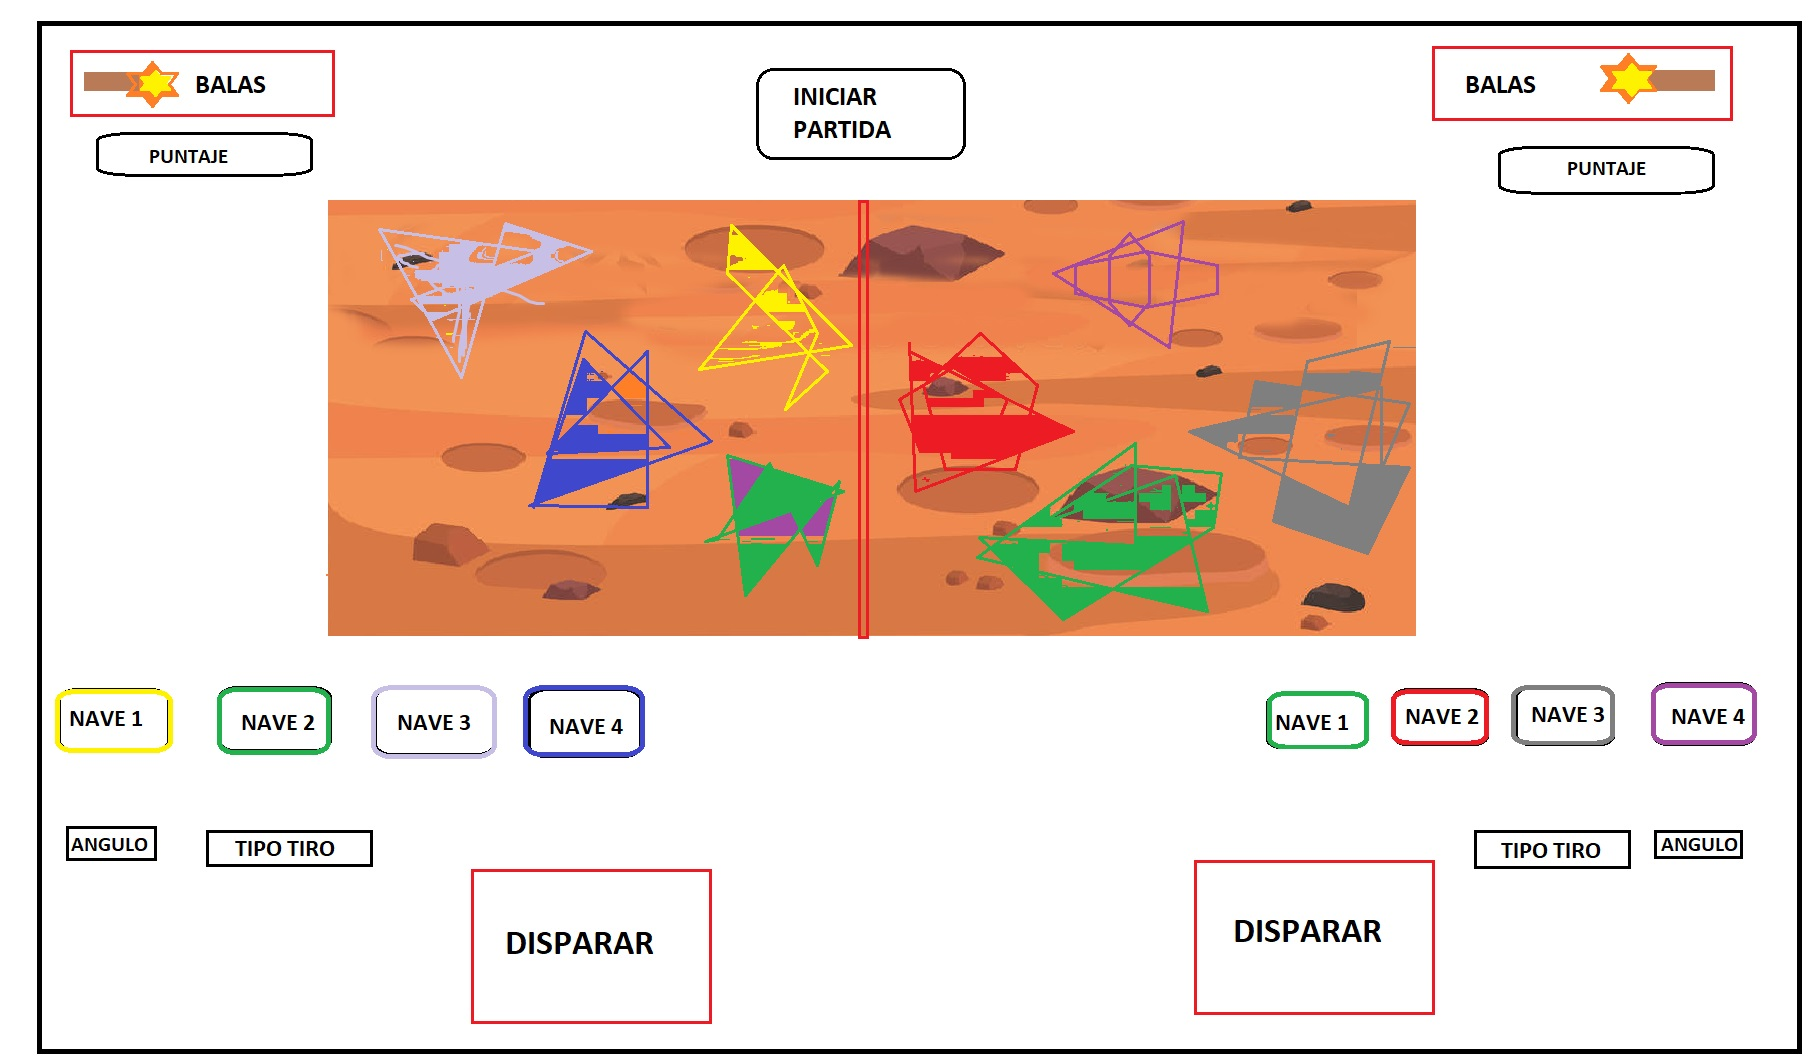
\includegraphics[width=15cm]{plantilla_latex/imagenes/esquema nemesis.png}
\centering
\caption{esquema Némesis}
\label{fig:cpplogo}
\end{figure}
La implementacion de un espacio fisico tri-dimensional o de dos dimensiones se tomara en cuenta a partir de la cantidad de memoria que se tenga a disposicion.


El juego constaria de unas partes las que son: mesa, barreras, porterias, puck(disco) y remos.

\section{ Imágenes de referencia} \label{imagenes}

En la Figura (\ref{fig:Batalla}), se muestra un imagen de juego Batalla naval del cual fue inspirado el juego Némesis

\label{imagenes}
\begin{figure}[h]
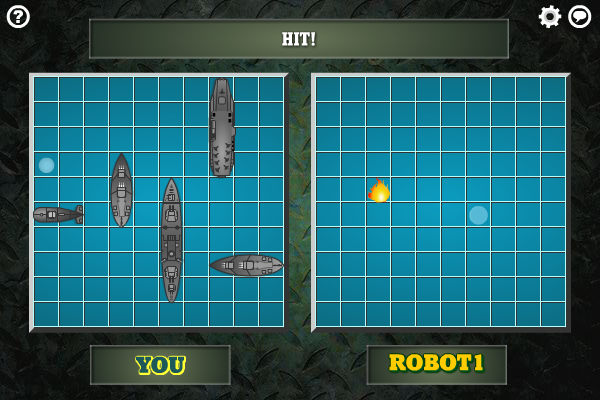
\includegraphics[width=10cm]{plantilla_latex/imagenes/Batalla naval.png}
\centering
\caption{Imagen de referencia}
\label{fig:Batalla}
\end{figure}


\end{document}
